\section{Numerical validation and implementation cost}
\label{sec:coordinate-validation}

The reproducible script \texttt{validation/verify\_coordinates.py} evaluates
four normalized toy machines at one common-purpose operating point per model.
The values are not a motor rating; they make cross-representation identities,
singular sets, and conditioning inspectable.

\begin{center}
\begin{tabular}{lrrrrr}
\toprule
Case & \(M\) & \(P_{\mathrm{Cu}}\) & \(U\) & \(\psi_s\) &
\(\kappa_2(J)\)\\
\midrule
SPM & 2.7060 & 0.1527 & 1.7712 & 0.8195 & 8.54\\
IPMSM & 2.2770 & 0.1695 & 1.4217 & 0.6396 & 6.20\\
linear EESM & 0.6300 & 0.3252 & 0.6956 & 0.2856 & 8.74\\
saturated EESM & 0.6246 & 0.3252 & 0.6693 & 0.2698 & 14.10\\
\bottomrule
\end{tabular}
\end{center}

For the two-current cases, \(J\) belongs to \((M,\psi_s)\); for EESM it
belongs to \((M,P_{\mathrm{Cu}},U)\). The saturated flux map bends the local
task frame and worsens this particular chart at the reported point. Across
the sampled domains, the largest finite condition numbers were
\(1.62\times10^3\) for the IPMSM chart and \(2.17\times10^4\) for the EESM
performance chart. The high values form curves near gradient dependence, not
uniform machine-wide penalties.

\begin{figure}[tb]
\centering
\begin{tikzpicture}
\begin{groupplot}[
 group style={group size=2 by 1,horizontal sep=1.1cm},
 width=.42\textwidth,height=5.4cm,
 xlabel={\(i_d\)},ylabel={\(i_q\)},
 point meta min=0,point meta max=4
]
\nextgroupplot[title={IPMSM: \((M,\psi_s)\)}]
\addplot[scatter,only marks,mark size=.85pt,scatter src=explicit]
 table[x=id,y=iq,meta=logcond]{figures/data/coordinate_condition_ipm.dat};
\nextgroupplot[title={EESM slice: \((M,P,U)\)},
 colorbar,colorbar style={ylabel={\(\log_{10}\kappa_2\)}}]
\addplot[scatter,only marks,mark size=.85pt,scatter src=explicit]
 table[x=id,y=iq,meta=logcond]{figures/data/coordinate_condition_eesm.dat};
\end{groupplot}
\end{tikzpicture}
\caption{Conditioning maps of candidate task charts. Warm/high-value bands are
places where inversion amplifies noise and a fallback chart is required.}
\label{fig:conditioning-maps}
\end{figure}


The symbolic suite proves the arbitrary-frame derivative, the active-flux
torque identity, the signed hyperbolic forward/inverse equations, and their
rate equations. The numerical suite returns a current round-trip error
\(1.57\times10^{-16}\), hyperbolic inverse error below printed precision, and
moving-frame derivative residual \(2.50\times10^{-8}\). Torque, copper loss,
and squared voltage agree before and after whitening/rotation to machine
precision. For the sampled linear EESM, the normalized torque--voltage
commutator is \(0.6702\), so exact joint diagonalization is excluded; the
simple offline Jacobi search reduces normalized off-diagonal energy from
\(1.2912\) to \(0.3230\).

\subsection{Reference operation-count model}

The following counts describe one illustrative EESM fast-loop evaluation,
excluding PWM and ADC hardware. A sin/cos pair counts as one CORDIC service;
the full \(3\times3\) solve is listed separately rather than hidden as scalar
operations. Compiler fusion, symmetry, fixed coefficients, and parallel FPGA
pipelines can change cycle counts, so these numbers compare algorithms, not
processors.

\begin{center}
\resizebox{\textwidth}{!}{%
\begin{tabular}{lrrrrrrrrrrr}
\toprule
Architecture & mult & add & div & sqrt & CORDIC & LUT & interp. & integ. &
PI & matrix solve & obs. states\\
\midrule
\(dq\) CVC & 32&24&0&0&1&2&2&3&3&0&0\\
\(ft\) DFVC & 42&30&1&1&2&0&0&4&2&0&2\\
active-flux CVC & 38&27&0&0&1&1&1&3&3&0&2\\
torque/flux IOFL & 72&52&3&0&1&0&0&3&3&1&2\\
\((i_T,\alpha,z_0)\) task control & 61&44&4&1&1&1&1&3&3&1&2\\
\bottomrule
\end{tabular}}
\end{center}

\begin{figure}[tb]
\centering
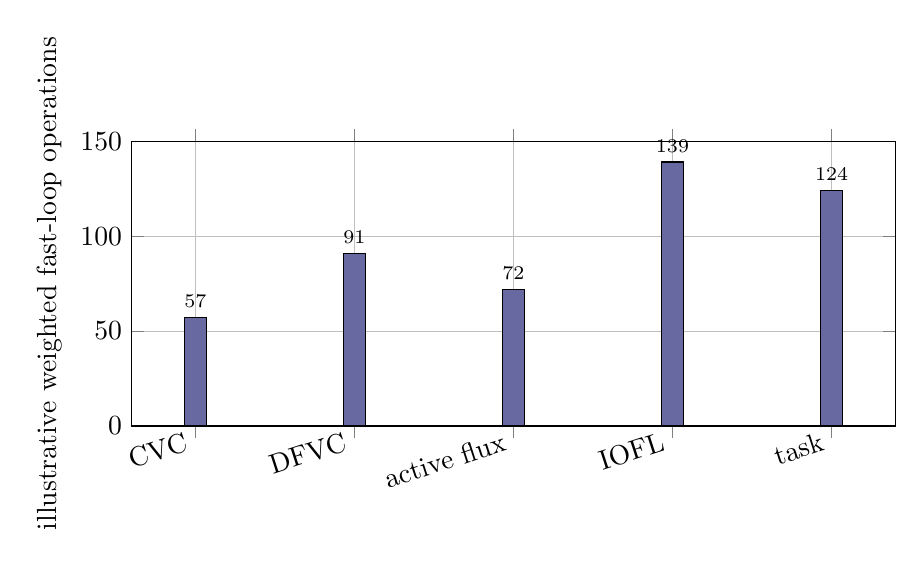
\begin{tikzpicture}
\begin{axis}[
 ybar,bar width=8pt,width=.93\textwidth,height=5.2cm,
 ylabel={illustrative weighted fast-loop operations},
 symbolic x coords={CVC,DFVC,active flux,IOFL,task},
 xtick=data,x tick label style={rotate=18,anchor=east},
 ymin=0,ymax=150,grid=major,
 nodes near coords,nodes near coords style={font=\scriptsize},
]
\addplot[fill=MidnightBlue!65] coordinates
 {(CVC,57) (DFVC,91) (active flux,72) (IOFL,139) (task,124)};
\end{axis}
\end{tikzpicture}
\caption{Weighted summary of the explicit count model
\((1\times\{\mathrm{mult,add,LUT}\},4\times\mathrm{div},
6\times\mathrm{sqrt},12\times\mathrm{CORDIC})\). Observer and matrix-solve
states are reported separately in the table and not hidden in these bars.}
\label{fig:operation-counts}
\end{figure}


State-dependent flux Jacobians need not be refreshed at the PWM rate. A
practical split evaluates transforms, PI laws, and voltage limiting in the
fast loop, while magnetic-map interpolation, Jacobian factorization, and
frame continuity checks run every \(N=4\ldots20\) samples when their variation
permits. Caching reduces average MCU cost; FPGA designs can pipeline the same
matrix products but divisions, square roots, and normalization remain the
fixed-point hazards. Close to a singular chart the dynamic range, not the
nominal multiplication count, is the decisive cost.

\begin{figure}[tb]
\centering
\begin{tikzpicture}[font=\small,>=Latex]
\node[draw,rounded corners,fill=MidnightBlue!8,minimum width=4.8cm,minimum height=2.4cm,align=center] (psm) at (0,0)
 {PSM/IPMSM\\2 current coordinates\\\(M=M_0\): 1-D curve\\one torque-neutral tangent};
\node[draw,rounded corners,fill=ForestGreen!9,minimum width=4.8cm,minimum height=2.4cm,align=center] (eesm) at (6.3,0)
 {EESM\\3 current coordinates\\\(M=M_0\): 2-D surface\\two torque-neutral tangents};
\draw[->,very thick] (psm)--node[above]{add field-current state and input}(eesm);
\draw[Purple,very thick] (-1.65,-1.75) .. controls (-.7,-1.1) and (.6,-2.3) .. (1.65,-1.55);
\draw[Purple!45,fill=Purple!8] (4.8,-2.15) .. controls (5.5,-1.25) and (6.7,-2.6) .. (7.8,-1.6)
 .. controls (7.1,-1.05) and (5.6,-1.0) .. cycle;
\end{tikzpicture}
\caption{Dimensionality of constant-torque sets. EESM redundancy supplies one
additional independent allocation direction.}
\label{fig:psm-eesm-nullspaces}
\end{figure}


\subsection{Sensors and observers are part of the bill}

\begin{center}
\begin{tabularx}{\textwidth}{lXXX}
\toprule
Method & measured/estimated quantities & main saved map & added sensitivity\\
\midrule
\(dq\) CVC & phase currents, rotor angle & none & parameter feedforward and reference maps\\
\(ft\) DFVC & currents, stator-flux vector/angle & field-weakening current map & flux integration and low-speed model\\
Active flux & currents, rotor angle or active-flux angle & machine-type torque formula & \(L_q\), flux map, observer offset\\
Performance chart & currents plus modelled \(M,P,U\) gradients & several references locally & inverse Jacobian conditioning\\
\bottomrule
\end{tabularx}
\end{center}

Removing Park rotation is not the objective: it is cheap on current hardware.
The relevant question is whether the \emph{whole stack} loses calibration
tables, reference generators, decoupling terms, or loops after observer and
inverse-map costs are included.
